\documentclass[11pt]{article}

% add some essential packages, some might not be used

\usepackage[T1]{fontenc} 
\usepackage[utf8]{inputenc}
\usepackage{xeCJK}
\usepackage[usenames,dvipsnames]{color}
\usepackage{natbib}
\usepackage{authblk}
\usepackage{ragged2e}
\usepackage{amsmath}
\usepackage[a4paper,margin=1in,bottom=1.0in]{geometry}
\usepackage{url}
\usepackage{array}
\usepackage{bbding}
\usepackage{amssymb}
\usepackage{graphicx}
\usepackage{adjustbox}
\usepackage{subcaption}
\usepackage{booktabs}
\usepackage{float}
\usepackage{appendix}
\usepackage{hyperref}
\usepackage{url}
\usepackage[english, greek]{babel}
\usepackage{adjustbox}
%\usepackage{enumitem}
\usepackage{textgreek}
\usepackage{tcolorbox}


\usepackage{listings}
\usepackage{wasysym}
\usepackage{amsthm}
\usepackage{framed}

\usepackage{rotating} % for the horizontal page table

\usepackage{tikz}
\usetikzlibrary{calc}
\usetikzlibrary{matrix}
\usetikzlibrary{positioning}
\usepackage{color}
\usepackage{setspace}
\usepackage{enumerate}
\usepackage{bm}


\usepackage{tcolorbox} % package for making colorful box 

 \setlength{\parskip}{0.15cm} % change the paragraph spacing 
\renewcommand\labelitemi{$\vcenter{\hbox{\tiny$\bullet$}}$} % set the bullet size as tiny 

% \newcommand*\rot{\rotatebox{90}} % for rotate text  

\usepackage{sectsty} %package for section size 

\sectionfont{\fontsize{14}{12}\selectfont} % Change the section font size

\subsectionfont{\fontsize{13}{12}\selectfont} 
\subsubsectionfont{\fontsize{12}{12}\selectfont}

\newcommand\numberthis{\addtocounter{equation}{1}\tag{\theequation}} % new command 

\newenvironment{remark}[2][\textit{Remark:}]{\begin{trivlist}
\item[\hskip \labelsep { #1}]}{\end{trivlist}}

\theoremstyle{definition}
\newtheorem{definition}[subsection]{Definition}
\newtheorem{proposition}[subsection]{Proposition}
\newtheorem{corollary}[subsection]{Corollary}
\newtheorem{theorem}[subsection]{Theorem}
\newtheorem{axiom}[subsubsection]{Axiom}
\newtheorem{lemma}[subsection]{Lemma}
\newtheorem{example}[subsection]{Example}
\newtheorem{hypothesis}[subsubsection]{Hypothesis}

\newcommand{\zn}{\mathbb{Z}}
\newcommand{\cn}{\mathbb{C}}
\newcommand{\qn}{\mathbb{Q}}
\newcommand{\rn}{\mathbb{R}}
\newcommand{\pn}{\mathbb{P}}
\newcommand{\fn}{\mathbb{F}}
\newcommand{\nn}{\mathbb{N}}
\usepackage{pythonhighlight}
\renewcommand{\arraystretch}{1.2}

\usepackage{courier}

\numberwithin{equation}{section}

\begin{document}

\selectlanguage{english}


\title{人工智能基础第二章实验}
\author{王斐 Michael}
\affil{SenseTime Edu}
\date{}

\maketitle

\section{前言}

这一章是人工智能基础的入门章节,即通过鸢尾花案例来介绍简单的感知器(perceptron)线性二元分类,并且引入支持向量机(support vector machine)模型的学习。在本章节的实验中,我们会通过不同的案例来,来学习和训练以下相关知识点:
\begin{itemize}
	\item 熟悉数据阵
	\item 向量运算和其几何性质
	\item 线性分类
	\item 梯度下降法(Gradient Descent)
	\item 感知器线性二元线性分类
	\item 支持向量机(support vector machine)二元线性线性分类
	\item 支持向量机(support vector machine)二元非线性分类(选修)
\end{itemize}

\section{实验重点}

同学们在进行本章的实验练习时,要留意下面几个要点:
\begin{enumerate}
	\item 摆脱计算思维,所有计算能扔给计算机的就扔给计算机
	\item 理解数学概念后,善于用计算机来直观得呈现相关概念
	\item 培养对数据阵的直观感受训练自己对机器学习模型的流程化理解,即 \begin{itemize}
		\item 数据准备和可视化
		\item 模型搭建和调用
		\item 模型运行寻找规律参数
		\item 模型预测和评估
	\end{itemize}
\end{enumerate}

提示: 只要你会解一元二次方程组,那么你就可以顺利完成该实验,所以请耐心做完(可以分三次,每次30分钟完成全部实验)
\begin{tcolorbox}[title=代码不可复制!]
	本实验内容所有代码需要同学们自己\textbf{输入},因为如果可以复制的话,你可能不会自己输入,也不会养成良好的编程习惯。
\end{tcolorbox}



\newpage

\section{实验1: 数据阵、向量和及其性质}

我们在课程中,学习了数据阵的定义,并且给出了下面的图形演示。
\begin{figure}[H]
	\centering
	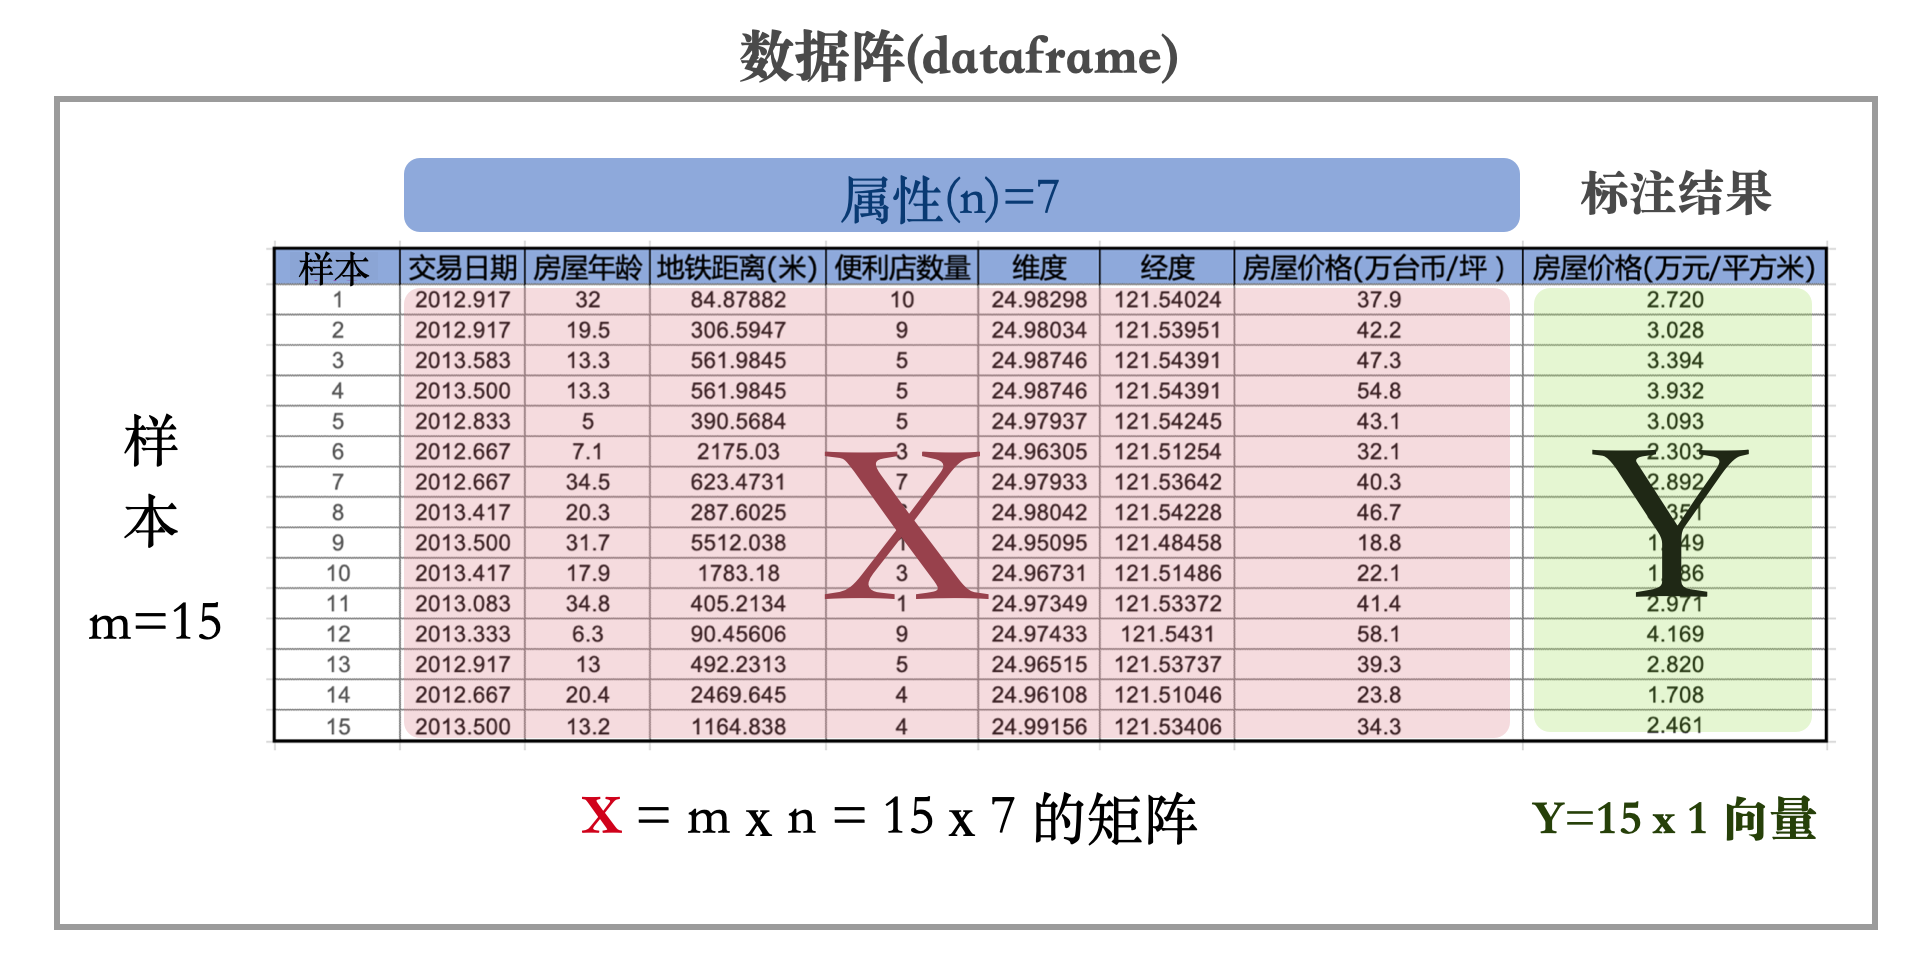
\includegraphics[width=0.9\textwidth]{/Users/Michael/Documents/MDLforBeginners/Chapter2/Lecture_slides/fig/dataframeVis.png}
	\caption{数据阵可视化}
\end{figure}
下面我们就来学习\texttt{Python}语言环境下的数据阵操作。按照惯例我们首先加载具体的工具包。有些工具包是辅助我们实验的,有些被标记\texttt{重点内容}的,需要同学们掌握。
\begin{python}
# 加载常用工具包,SenseStudy 目前测试可以加载下列工具包
# 注意,非重点内容不需要掌握
import numpy as np  #重点内容
import pandas as pd  #重点内容
import matplotlib.pyplot as plt  #重点内容
import seaborn as sns
from sklearn import datasets
from sklearn import preprocessing
from sklearn.model_selection import train_test_split
from sklearn.linear_model import Perceptron
\end{python}

\subsection{鸢尾花数据阵构造和读取}
\begin{python}
iris = datasets.load_iris()  # 加载数据阵
print(iris.data[0: 5])
print(iris.target[0:5])
print(iris.feature_names) 
iris.feature_names.append('Category')
iris_df = pd.DataFrame(np.column_stack((iris.data, iris.target)),
                       columns=iris.feature_names)
iris_df.Category = iris_df.Category.astype(int)
print(iris_df.shape)  # 150 x 5 dataframe, 特征变量矩阵X 为 150 x 4, 即150 个样本, 4个属性, 还有1个结果向量 
\end{python}


\subsection{鸢尾花数据阵可视化}
\begin{python}
sns.set(style="whitegrid")  
fig, axes = plt.subplots(1, 2, figsize=(12, 6))
sns.scatterplot(x=iris_df.iloc[:, 0],
                y=iris_df.iloc[:, 1],
                hue=iris_df.iloc[:, 4],
                ax=axes[0], s=80, palette="Set1")
sns.scatterplot(x=iris_df.iloc[:, 2],
                y=iris_df.iloc[:, 3],
                hue=iris_df.iloc[:, 4],
                ax=axes[1], s=80, palette="Set1")
\end{python}


\subsection{鸢尾花种类选取}

现在我们选取两种鸢尾花,并且只对其花瓣的长度和宽度进行可视化。
\begin{python}
iris_df_binary = iris_df[iris_df.Category != 1]  # 选取种类标记为 0 和 2 的鸢尾花
print(iris_df_binary.shape)  # 查看新的维数
print(iris_df_binary.columns)  # 查看属性名称
sns.scatterplot(x=iris_df_binary.iloc[:, 2],
                y=iris_df_binary.iloc[:, 3],
                hue=iris_df_binary.iloc[:, 4],
                s=80, palette="Set1")  # 只对两种鸢尾花进行可视化
\end{python}














\end{document}